\documentclass[sigplan,review,nonacm,9pt]{acmart}

\usepackage{minted}
\usepackage{makecell}
\usepackage{booktabs}
\graphicspath{ {./figs/} }

% https://tex.stackexchange.com/questions/655620/how-to-make-acmart-stop-complaining-about-missing-country-in-affiliation
\makeatletter
\def\@ACM@checkaffil{% Only warnings
    \if@ACM@instpresent\else
    \ClassWarningNoLine{\@classname}{No institution present for an affiliation}%
    \fi
    \if@ACM@citypresent\else
    \ClassWarningNoLine{\@classname}{No city present for an affiliation}%
    \fi
    \if@ACM@countrypresent\else
        \ClassWarningNoLine{\@classname}{No country present for an affiliation}%
    \fi
}
\makeatother

%%
%% \BibTeX command to typeset BibTeX logo in the docs
\AtBeginDocument{%
  \providecommand\BibTeX{{%
    Bib\TeX}}}

%% Rights management information.  This information is sent to you
%% when you complete the rights form.  These commands have SAMPLE
%% values in them; it is your responsibility as an author to replace
%% the commands and values with those provided to you when you
%% complete the rights form.
\setcopyright{acmcopyright}
\copyrightyear{2023}
\acmYear{2023}
%\acmDOI{XXXXXXX.XXXXXXX}

%% These commands are for a PROCEEDINGS abstract or paper.
\acmConference[PLARCH '23]{PLARCH 2023}{June 17, 2023}{Orlando, FL}
%%
%%  Uncomment \acmBooktitle if the title of the proceedings is different
%%  from ``Proceedings of ...''!
%%
%%\acmBooktitle{Woodstock '18: ACM Symposium on Neural Gaze Detection,
%%  June 03--05, 2018, Woodstock, NY}
%\acmPrice{15.00}
%\acmISBN{978-1-4503-XXXX-X/18/06}


%%
%% Submission ID.
%% Use this when submitting an article to a sponsored event. You'll
%% receive a unique submission ID from the organizers
%% of the event, and this ID should be used as the parameter to this command.
%%\acmSubmissionID{123-A56-BU3}

%%
%% For managing citations, it is recommended to use bibliography
%% files in BibTeX format.
%%
%% You can then either use BibTeX with the ACM-Reference-Format style,
%% or BibLaTeX with the acmnumeric or acmauthoryear sytles, that include
%% support for advanced citation of software artefact from the
%% biblatex-software package, also separately available on CTAN.
%%
%% Look at the sample-*-biblatex.tex files for templates showcasing
%% the biblatex styles.
%%

%%
%% The majority of ACM publications use numbered citations and
%% references.  The command \citestyle{authoryear} switches to the
%% "author year" style.
%%
%% If you are preparing content for an event
%% sponsored by ACM SIGGRAPH, you must use the "author year" style of
%% citations and references.
%% Uncommenting
%% the next command will enable that style.
%%\citestyle{acmauthoryear}
\settopmatter{printacmref=false}

%%
%% end of the preamble, start of the body of the document source.
\begin{document}

%%
%% The "title" command has an optional parameter,
%% allowing the author to define a "short title" to be used in page headers.
\title{Separating Description from Interpretation}
\subtitle{Functional-Esque APIs for Hardware Design and Verification}

%%
%% The "author" command and its associated commands are used to define
%% the authors and their affiliations.
%% Of note is the shared affiliation of the first two authors, and the
%% "authornote" and "authornotemark" commands
%% used to denote shared contribution to the research.
\author{Vighnesh Iyer}
\email{vighnesh.iyer@berkeley.edu}
\orcid{0000-0001-6934-6577}
\affiliation{%
  \institution{UC Berkeley}
}

\author{Borivoje Nikolić}
\email{bora@eecs.berkeley.edu}
\orcid{0000-0003-2324-1715}
\affiliation{%
  \institution{UC Berkeley}
}


%%
%% By default, the full list of authors will be used in the page
%% headers. Often, this list is too long, and will overlap
%% other information printed in the page headers. This command allows
%% the author to define a more concise list
%% of authors' names for this purpose.
% \renewcommand{\shortauthors}{Trovato et al.}

\begin{abstract}
Over the past few decades, many hardware design languages (e.g. Lava, Chisel, PyMTL3) have been implemented as DSLs embedded in a general purpose programming language.
This approach takes advantage of the host language`s features and ecosystem, such as its type system, libraries, build tools, IDEs, and unittest frameworks.
We make the case that embedded DSLs are an ideal platform for hardware design languages, by leveraging them to build \textit{functional APIs} for RTL simulation, stimulus generation, temporal property specification, and FSM construction.
We invite discussion on what other primitives can be embedded in a general-purpose language to enhance RTL design and verification.
% we're already familiar with this concept for HDLs implemented as eDSLs - but where else can we use this concept? I demonstrate 3 use cases: simcommand, parametric generators, sequences, recipes
% embedding is not only good because of ecosystem, but also because it allows you to leverage features of the host language like its FP support
%compared to freestanding DSLs or custom compilers.
%I make the case that this approach is good and can be applied to even more areas!
%What else can we embed to enable more expressive or performant hardware design and verification?
\end{abstract}

% \received{20 February 2007}
% \received[revised]{12 March 2009}
% \received[accepted]{5 June 2009}

\maketitle

\section{Functional Principles}
% ADTs
% Separating description from interpretation + combinators
% Customizable interpreters
% This technique has been applied to RTL-level HW design, but what other areas can we apply this to?

Building APIs on the practical foundations of functional programming provides several benefits beyond the mostly theoretical notions of referential transparency.
Importantly, functional APIs seperate \textit{what to do} (the description) from \textit{how it is done} (the interpreter).

This notion is already well understood in the context of HDLs implemented as eDSLs.
eDSLs embed hardware primitives (datatypes, registers, memories, logical / arithmetic operators) and `connection' primitives (modules, IO ports, wires, bindings) in the host language as a set of algebraic datatypes (ADTs).
The RTL designer instantiates the primitives and connects them together with a normal program written in the host language.
Here, \textit{the description}, is an in-memory representation of a circuit that is constructed when the program is executed, while \textit{the interpreter} turns that representation into some output (e.g. FIRRTL, Circt IR, Verilog, SMT, btor).

The same principle of separating description from interpretation has many other useful applications in hardware design and verification, albeit with different primitives and interpreters.

%\section{SimCommand: Functional Testbench API}
\section{A Functional Testbench API}

While you can write testbenches in SystemVerilog for any circuit generated from embedded HDLs, it is more ergonomic to write testbenches in the same host language you use to write RTL, so you can share parameters and exploit the features of the host language.
However, existing testbench APIs, such as chiseltest and cocotb (\textbf{cite}), suffer from poor performance due to their implementation of the \texttt{fork/join} primitive used to express testbench parallelism.
We propose a functional eDSL and API, SimCommand (\textbf{cite}), which achieves fast \texttt{fork/join} by embedding testbench primitives in Scala and separating testbench description and interpretation.

\begin{figure}
\begin{minted}[breaklines,fontsize=\small]{scala}
// A pure functional description of a testbench action
def dequeue[T](io: DecoupledIO[T]): Command[T] = for {
    _ <- waitUntil(io.valid, 1)
    _ <- poke(io.ready, 1)
    value <- peek(io.bits)
    _ <- step(1)
} yield value

// Actually running the Command with unsafeRun
val v = dequeue(queue.io).unsafeRun(queue.clock)
\end{minted}
\caption{A \textit{description} of dequeuing data from a ready-valid interface, followed by invoking the interpreter to \textit{run} that description in RTL simulation using the SimCommand interpreter}
\label{fig:simcommand}
\end{figure}

\begin{figure}
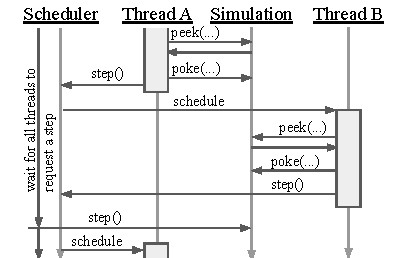
\includegraphics[scale=1]{simcommand/scheduler.pdf}
\caption{Scheduling simulation threads on a single executor thread in the SimCommand interpreter}
\label{fig:simcommand_interp}
\end{figure}

\begin{figure*}
\textbf{add cites for each base type}
\begin{tabular}{p{2.5cm}p{5cm}p{3cm}p{4cm}}\toprule
ADT Base Type & ADT Primitives / Combinators & Composition Primitives & Interpreter Result\\\midrule
\mintinline[]{scala}{Data} & \texttt{UInt}, \texttt{SInt} (base hardware datatypes) \newline \texttt{Bundle}, \texttt{Vec} (aggregate types) \newline \texttt{Mux}, \texttt{+}, \texttt{|}, $\dots$ (operators) \newline \texttt{Reg}, \texttt{SyncReadMem} (state types) & \texttt{Module}, \texttt{Input}, \texttt{Output}, \texttt{Wire}, \texttt{:=} (connect) & FIRRTL representation of the circuit\\\midrule
\mintinline[]{scala}{Command[R]} & \texttt{Poke}, \texttt{Peek}, \texttt{Step} (basic testbench ops) \newline \texttt{Fork}, \texttt{Join} (simulation threading) \newline \texttt{MakeChannel}, \texttt{Put}, \texttt{Get} (channels) & Monadic bind & Interaction with an RTL simulator terminating with a value of type \texttt{R}\\\midrule
\mintinline[]{scala}{Gen[A]} & \texttt{uniform}, \texttt{range}, \texttt{normal}, \texttt{oneOf} & Monadic bind & Values of type \texttt{A} conforming to the generative constraints\\\midrule
\mintinline[]{scala}{Property[T, S]} & \texttt{AtomicProp}, \texttt{||}, \texttt{\&\&}, \texttt{|->} & \texttt{Concat}, \texttt{Intersect} & Monitor automaton for the \texttt{Property} using local state \texttt{S} $^{(\ast)}$ over traces of type \texttt{T} $^{(\ast)}$\\\midrule
\mintinline[]{scala}{Recipe} & \texttt{action}, \texttt{tick}, \texttt{fork} $^{(\ast)}$ & \texttt{sequential}, \texttt{while}, \texttt{ifThenElse} & Chisel RTL circuit that implements the imperative \texttt{Recipe} \\
\bottomrule
\end{tabular}
\caption{Overview of the primitives and generated output of eDSLs in the Chisel HDL ecosystem. {\small $^{(\ast)}$ = hypothetical / incomplete implementation}}
\end{figure*}

Other implementations use JVM threads and mutexes (chiseltest) or Python's async/await coroutines (cocotb) to implement \texttt{fork/join} simulation threads.
These techniques cannot keep up with the high frequency of suspend/resume operations in simulation threads.
In contrast, SimCommand uses monadic composition of testbench primitives (\textbf{cite hardcaml\_step\_tb}) to implement cooperatively yielding simulation threads that can suspend/resume quickly.

The core datatype of SimCommand is \texttt{Command[R]}, which describes a testbench operation that eventually terminates with a value of type \texttt{R}.
The primitives include testbench operations such as \texttt{peek} and \texttt{poke} to sense and drive RTL signals, \texttt{step} to advance the clock, and \texttt{fork} and \texttt{join} to implement simulation threads.
See the example in Figure \ref{fig:simcommand} which demonstrates Scala's for-comprehension syntax for composing \texttt{Command} primitives and the \textit{separation of description and interpretation}.

The SimCommand interpreter works as shown in Figure \ref{fig:simcommand_interp}: on every timestep, each thread, stored as a pointer to a \texttt{Command}, is run until it hits a \texttt{step} or \texttt{join} (a yield point).
Once all threads have run to their yield point, and all recursively spawned threads have done the same, the scheduler steps the clock in the underlying RTL simulator, and repeats until the main thread terminates.

SimCommand has several other features such as channels for inter-thread communication, cycle skipping optimizations, and runtime checks for thread order dependencies.
Separating description and interpretation yields an API that's 5-30x faster than cocotb and chiseltest, while being purely functional.

% Advantages:
% Fast fork/join
% Cycle skipping
% Deterministic channels
% Instrumentation to Verilog testbench built into interpreter
% Fixpoint iteration
% Catching thread ordering issues at runtime


\section{Conclusion}
% Leverage Scala's for-comprehension (similar to Haskell's do-notation) for monadic composition.

\begin{acks}
The example libraries in this paper are worked on by: Young-Jin Park, Rohit Agarwal, Andy Lin, and Bryan Ngo.
TODO: ask Bora for other acks.
\end{acks}

\bibliographystyle{ACM-Reference-Format}
\bibliography{references}

% \appendix

\end{document}
\endinput
